\documentclass{sigchi-ext}
% Please be sure that you have the dependencies (i.e., additional
% LaTeX packages) to compile this example.
\usepackage[T1]{fontenc}
\usepackage{textcomp}
\usepackage[scaled=.92]{helvet} % for proper fonts
\usepackage{graphicx} % for EPS use the graphics package instead
\usepackage{balance}  % for useful for balancing the last columns
\usepackage{booktabs} % for pretty table rules
\usepackage{ccicons}  % for Creative Commons citation icons
\usepackage{ragged2e} % for tighter hyphenation

% \usepackage{marginnote} \usepackage[shortlabels]{enumitem}
% \usepackage{paralist}

% EXAMPLE BEGIN -- HOW TO OVERRIDE THE DEFAULT COPYRIGHT STRIP --
 \copyrightinfo{Permission to make digital or hard copies of all or
 part of this work for personal or classroom use is granted without
 fee provided that copies are not made or distributed for profit or
 commercial advantage and that copies bear this notice and the full
 citation on the first page. Copyrights for components of this work
 owned by others than ACM must be honored. Abstracting with credit is
 permitted. To copy otherwise, or republish, to post on servers or to
 redistribute to lists, requires prior specific permission and/or a
 fee. Request permissions from permissions@acm.org.\\
 {\emph{CHI'14}}, April 26--May 1, 2014, Toronto, Canada. \\
 Copyright \copyright~2014 ACM ISBN/14/04...\$15.00. \\
 DOI string from ACM form confirmation}
% EXAMPLE END

\title{Study Social: Forming Study Groups Online Through Social Media}

\numberofauthors{4}
% Notice how author names are alternately typesetted to appear ordered
% in 2-column format; i.e., the first 4 autors on the first column and
% the other 4 auhors on the second column. Actually, it's up to you to
% strictly adhere to this author notation.
\author{%
  \alignauthor{%
    \textbf{Kai Anderson}\\
    \affaddr{Utah State University} \\
    \affaddr{Logan, UT 84321, USA} \\
    \affaddr{kai.andersom@gmail.com} }\alignauthor{%
    \textbf{Erik Falor}\\
    \affaddr{Utah State University} \\
    \affaddr{Logan, UT 84321, USA} \\
    \email{ewfalor@gmail.com} } \vfil \alignauthor{%
    \textbf{Maur\'{i}el Ramirez}\\
    \affaddr{Utah State University} \\
    \affaddr{Logan, UT 84321, USA} \\
    \email{mauriel.ramirez@gmail.com} }\alignauthor{%
    \textbf{Alan Williams}\\
    \affaddr{Utah State University} \\
    \affaddr{Logan, UT 84321, USA} \\
    \email{alan.williams@aggiemail.usu.edu} } \vfil  }




% Paper metadata (use plain text, for PDF inclusion and later
% re-using, if desired)
\def\plaintitle{Study Social: Forming Study Groups Online Through Social Media} \def\plainauthor{Kai Anderson, Erik Falor, Maur\'{i}el Ramirez, Alan Williams}
\def\plainkeywords{
	Social Media; Study Groups; Study Habits; Dating Service}
\def\plaingeneralterms{Documentation, Standardization}

%% Set up our PDF with metadata
\hypersetup{%
  pdftitle={\plaintitle}, pdfauthor={\plainauthor},
  pdfkeywords={\plainkeywords}, }

% \reversemarginpar%

\begin{document}

\maketitle

% Uncomment to disable hyphenation (not recommended)
% https://twitter.com/anjirokhan/status/546046683331973120
\RaggedRight{}

% Do not change the page size or page settings.
\begin{abstract}
Study Social is a mobile application designed to bring students together for
collaborative work and study. There are many benefits to studying in groups:
study groups help reduce procrastination, improve accuracy covering material,
increase the number of perspectives, and groups are more effective at
overcoming challenging material. While there are many benefits
to group study and collaboration some students are hesitant to forming new
groups based on past bad experiences or social barriers. While creating
this mobile application we specifically focused on creating a complete
solution for students looking for group collaboration and focused on
overcoming social barriers preventing the formation of groups. In this
paper we describe the methodology of our design and walk through of the
Study Social application.
\end{abstract}

\keywords{\plainkeywords}

\category{H.1.2}{User/Machine Systems}{Human factors, Software psychology}
\category{H.5.2}{User Interfaces}{Graphical user interfaces, prototyping, User-centered design, Interaction styles}
\category{H.5.3}{Groups and Organization Interfaces}{Asynchronous interaction, Collaborative computing, Computer-supported cooperative work, Organizational design, Web-based interaction}

\section{Introduction}

Beginning the development of the Study Social app, our group identified the
need within the user base of students to have a tool for collaborating and
group study. While the app has a broad application, the initial purpose was to
help students find groups. Beyond finding groups to study with Study Social
helps organize the group effort and provide tools like chat and file uploads
for the groups to work with.

Our initial problem statement when we began our research was, ``College
students seeking a compatible study group or tutor face a challenge as
difficult as finding a date''. While the initial problem statement is still
valid, helping students form groups and collaborate with students that begin
as possible strangers is more complicated.

Through our initial research dealing with student study habits and experiences
in study groups we found students are hesitant to join a study group based on
past experiences and usually prefer to work through difficult material on
their own than to form a study group. Several barriers include; group
socialized too much because of size, mismatched knowledge levels (one always
teaching the other), or the group was created by a professor and the group
members had different levels of motivation - to name a few.

Generally our interviewed students have had good experiences but the risk of
incompatibility outweighs the benefits to group study leading to individual
study. Petress indicates the benefits of group study as; increases confidence,
improves student’s subject articulation, increases perspective, validates
knowledge, etc. \cite{petress2004benefits}. In order to make a successful
application we began our work overcoming social barriers to forming a group
while creating a tool to help students take advantage of the benefits of group
study. Creating a platform to include setting up a profile for interactions,
finding a group (joining or creating a group), interacting with the group in a
meaningful ways (events, chat, and file upload).



\marginpar{%
  \vspace{-45pt} \fbox{%
    \begin{minipage}{0.925\marginparwidth}
      \textbf{Good Utilization of the Side Bar} \\
      \vspace{1pc} \textbf{Preparation:} Do not change the margin
      dimensions and do not flow the margin text to the
      next page. \\
      \vspace{1pc} \textbf{Materials:} The margin box must not intrude
      or overflow into the header or the footer, or the gutter space
      between the margin paragraph and the main left column. The text
      in this text box should remain the same size as the body
      text. Use the \texttt{{\textbackslash}vspace{}} command to set
      the margin
      note's position. \\
      \vspace{1pc} \textbf{Images \& Figures:} Practically anything
      can be put in the margin if it fits. Use the
      \texttt{{\textbackslash}marginparwidth} constant to set the
      width of the figure, table, minipage, or whatever you are trying
      to fit in this skinny space.
    \end{minipage}}\label{sec:sidebar} }



\section{Literature Review}
KAI ANDERSON KAI ANDERSON KAI ANDERSON KAI ANDERSON KAI ANDERSON
``An expert neural network system for dynamic job shop scheduling''~\cite{sim1994expert}
nec, vulputate eget, arcu. In enim justo, rhoncus ut, imperdiet a,
``Too much information''~\cite{christensen2006too}
venenatis vitae, justo. Nullam dictum felis eu pede mollis pretium.
``Real-time recommendations for user-item streams''~\cite{lommatzsch2015real}
Integer tincidunt. Cras dapibus. Vivamus elementum semper nisi. Aenean
``Love me Tinder: Untangling emerging adults' motivations for using the dating application Tinder''~\cite{sumter2017love}
vulputate eleifend tellus. Aenean leo ligula, porttitor eu, consequat
``Interaction-based collaborative filtering methods for recommendation in online dating''~\cite{krzywicki2010interaction}
vitae, eleifend ac, enim. Aliquam lorem ante, dapibus in, viverra quis,
``Binder: the Tinder for Studying''~\cite{binder}



\section{Investigative Research}
ALAN WILLIAMS ALAN WILLIAMS ALAN WILLIAMS ALAN WILLIAMS ALAN WILLIAMS
feugiat a, tellus. Phasellus viverra nulla ut metus varius laoreet.
Quisque rutrum. Aenean imperdiet. Etiam ultricies nisi vel augue.
Curabitur ullamcorper ultricies nisi. Nam eget dui.
Etiam rhoncus. Maecenas tempus, tellus eget condimentum rhoncus, sem
quam semper libero, sit amet adipiscing sem neque sed ipsum. Nam quam

\begin{figure}
  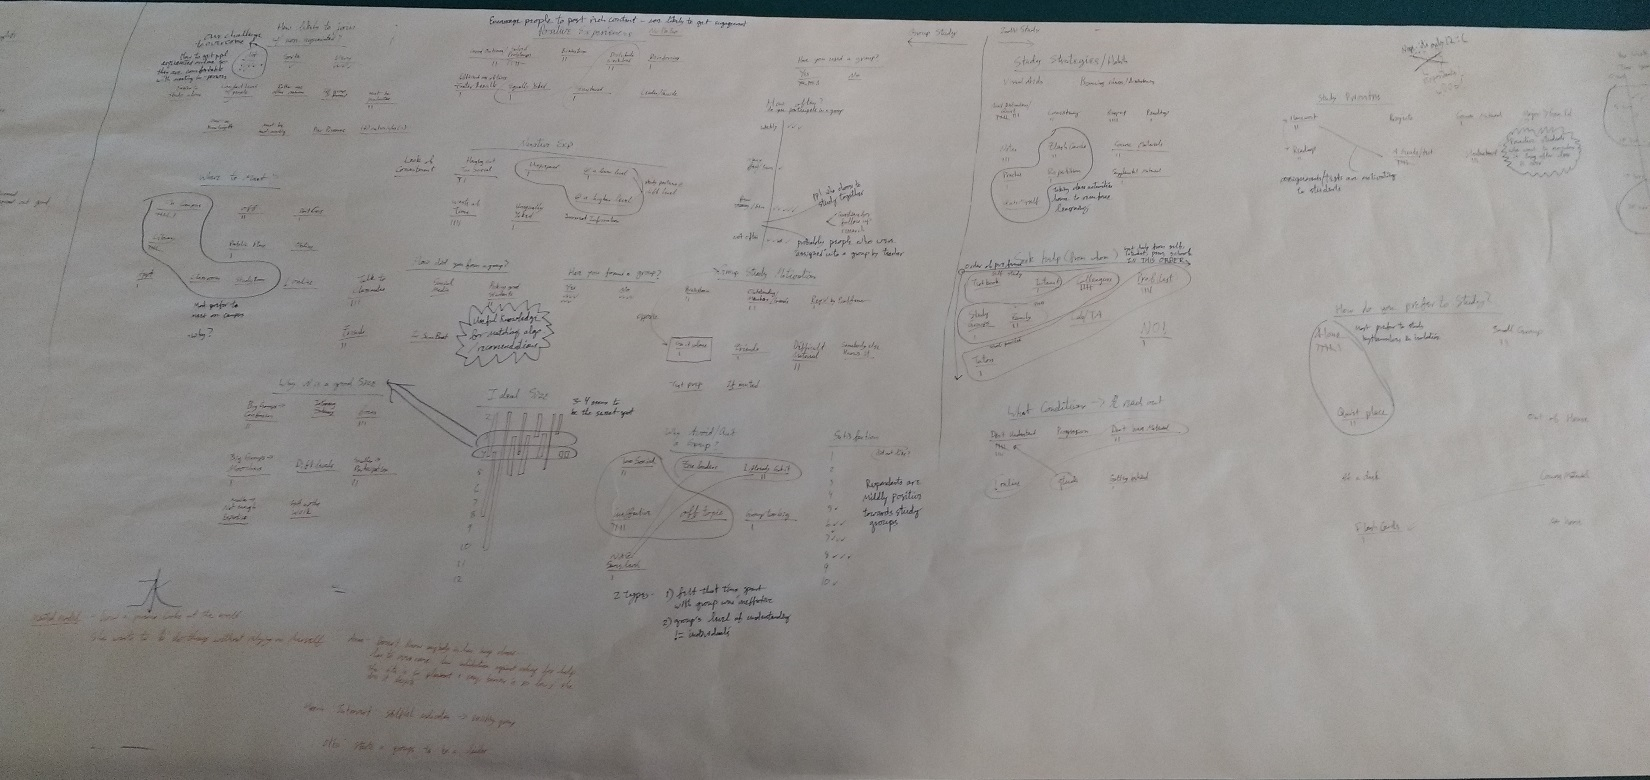
\includegraphics[width=0.9\columnwidth]{figures/affinity_diagram.jpg}
  \caption{Affinity diagram}~\label{fig:sample}
\end{figure}

\begin{marginfigure}[-15pc]
  \begin{minipage}{\marginparwidth}
    \centering
    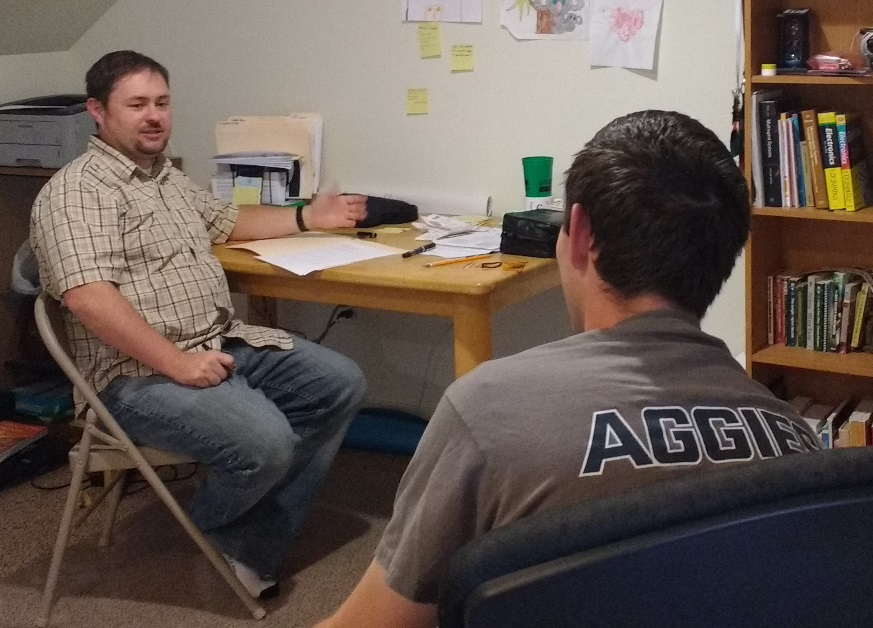
\includegraphics[width=0.9\marginparwidth]{figures/user_study.jpg}
    \caption{A user study was undertaken as one-on-one interviews with 12 subjects.}~\label{fig:marginfig}
  \end{minipage}
\end{marginfigure}



\section{Personas and Scenarios}
ALAN WILLIAMS ALAN WILLIAMS ALAN WILLIAMS ALAN WILLIAMS ALAN WILLIAMS
\textbf{TODO:}
\textit{Let's find some photographs to go a long with each of our personas.
We can throw that over into the gutter}
quam semper libero, sit amet adipiscing sem neque sed ipsum. Nam quam
nunc, blandit vel, luctus pulvinar, hendrerit id, lorem. Maecenas nec
odio et ante tincidunt tempus. Donec vitae sapien ut libero venenatis
faucibus. Nullam quis ante. Etiam sit amet orci eget eros faucibus
tincidunt. Duis leo. Sed fringilla mauris sit amet nibh. Donec sodales
sagittis magna. Sed consequat, leo eget bibendum sodales, augue velit

\marginpar{\vspace{5pc}So long as you don't type outside the right
  margin or bleed into the gutter, it's okay to put annotations over
  here on the left, too. You'll have to manually align the margin
  paragraphs to your \LaTeX\ floats using the
  \texttt{{\textbackslash}vspace{}} command.}



\subsection{Paper Prototype}

Our design process began by sketching several concepts out on paper. We refined
these sketches through a number of iterations, all the while keeping in balance
competing design considerations.

Working on paper allowed us to quickly explore several diverse structures and
layouts until we found one which we felt would be simple and intuitive. At this
stage we focused on design such principles as explorability and simplicity.
Knowing the time pressures which students face, we aimed to craft an experience
that wold be fun, inviting and, above all, efficient. We reasoned that a
demanding interface would be a turn off to the busy students we are trying to
reach.


\subsection{Digital Prototype}

After settling on a concept we created a digital prototype using the JustInMind Prototyping
tool~\cite{justinmind}. This software program enabled our team to create a hi-fidelity interactive
prototype with the ease of making a drawing. The JustInMind Prototyping tool supplies built-in
templates for designing both desktop and mobile applications. Realizing that digital content is
mostly consumed on mobile devices, we focused our efforts on creating a mobile prototype. With this
tool we were quickly able to produce a working prototype which brought to life our paper drawings.


\subsection{Cognitive Walk-through}

Members of our team guided four participants through a cognitive walk-through
evaluation. Participants were asked to complete a few simple, pre-defined tasks
using the digital prototype from a web browser. Having an interactive
web-based prototype made administering the cognitive walk-through simple owing
to the fact that our test subjects were already comfortable with the concept of
a webpage and could begin tackling their assigned tasks with minimal prompting.

The tasks assigned included creating and populating a personal profile, finding an existing study
group and creating a new study group. As participants completed these tasks they vocalized their
thoughts and frustrations so that we cold better understand the thought process of a typical user.

The cognitive walk-through revealed weaknesses in our design which we had theretofore been blind to.
One such revelation was that our navigation scheme was insufficient and inconsistent, leaving users
lost and confused.

This design deficit followed from our understanding of how a paper prototype
ought to be designed. Looking back, it is clear that we had come to envision
the application as a sequence of hyperlinked pages, one screen in size instead
of imagining it as a unified, continuous flow.  Navigation was unnecessarily
difficult because it wasn't always clear on which screen a piece of desired
information was located, nor was it obvious how to reach a desired destination
from the user's current screen.

Another issue reported by a majority of participants was inadequate feedback.
An oft-cited complaint was that after painstakingly entering data into the
mobile application via an on-screen keyboard, there was no "save" button
provided. Navigating back to the previous screen did not reassure the user that
their data was saved. Nor was there any indication of an autosave feature.
Because of this users sought in vain for the missing button and were reluctant
to leave the page containing the text-entry forms.

An evaluation of the results of this cognitive walk-through was subsequently
performed and recorded by team members.


\subsection{Heuristic evaluation}

Following the cognitive walk-through our team performed a heuristic evaluation on the most important
functions of the application. Of the ten design heuristics under consideration, two repeatedly came
up as problematic to our prototype. These were ``User control and freedom'' and ``consistency and
standards''. The aforementioned navigation confusion along with the lack of a save button were the
biggest drivers of the former heuristic. The latter was exemplified by our inconsistent use of
navigation hints and our over-complicated search interface.



\section{Usability Testing}

The result of the foregoing evaluation activities was a bottom-up redesign of
our application prototype which was prepared for a usability testing activity.



\begin{marginfigure}[-55pc]
	\begin{minipage}{\marginparwidth}
		\centering
		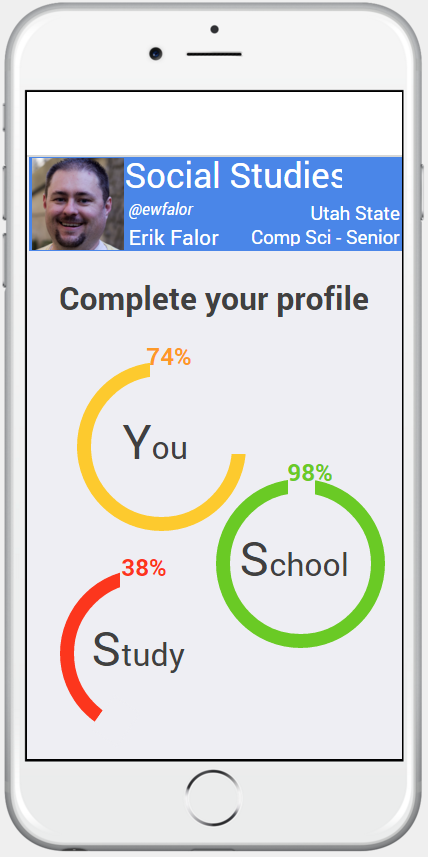
\includegraphics[width=0.9\columnwidth]{figures/prototype1.png}
		\caption{Profile landing page of the initial prototype}~\label{fig:prototype}
	\end{minipage}
\end{marginfigure}



\section{Usability Testing}

ERIK FALOR ERIK FALOR ERIK FALOR ERIK FALOR ERIK FALOR ERIK FALOR ERIK FALOR

The outcome of the cognitive walk-through and heuristic evaluation activities was a new and
more-refined prototype which was prepared for a round of usability tests.


luctus et ultrices posuere cubilia Curae; Sed aliquam, nisi quis
porttitor congue, elit erat euismod orci, ac placerat dolor lectus quis
orci. Phasellus consectetuer vestibulum elit. Aenean tellus metus,
bibendum sed, posuere ac, mattis non, nunc. Vestibulum fringilla pede
sit amet augue. In turpis. Pellentesque posuere. Praesent turpis.



\section{Conclusions}
KAI ANDERSON KAI ANDERSON KAI ANDERSON KAI ANDERSON KAI ANDERSON
luctus et ultrices posuere cubilia Curae; In ac dui quis mi
consectetuer lacinia.
Nam pretium turpis et arcu. Duis arcu tortor, suscipit eget, imperdiet
nec, imperdiet iaculis, ipsum. Sed aliquam ultrices mauris. Integer
ante arcu, accumsan a, consectetuer eget, posuere ut, mauris. Praesent



\section{Acknowledgements}
We are grateful to all of the participants who volunteered through interviews,
cognative walkthroughs, usability tests and in other activities. Their input
was invaluable and really helped this project take shape.
We owe a debt of gratitude to our helpful and enthusiastic mentor and advisor,
Dr. Amanda Hughes. We could never have created such a successful prototype
without her brilliant insight and helpful advice.
Some of the references cited in this paper are included for illustrative purposes only.



\balance{}

% \bibliographystyle{ACM-Reference-Format-Journals}
\bibliographystyle{SIGCHI-Reference-Format}
% \bibliographystyle{acm}
\bibliography{Team-FTW-Report}

\end{document}

%%% Local Variables:
%%% mode: latex
%%% TeX-master: t
%%% End:
